\section{问题一的模型建立与求解}

\subsection{统一储能模型}

储能允许范围为 $[1200,10800]~\mathrm{kWh}$。每个区间最大充、放电量为
\[
5000\times\frac{1}{6}=833.3333~\mathrm{kWh}.
\]
以 $c_t$ 表示母线送入电池的电量，
$r_t$ 表示电池送至母线的电量，则
\begin{equation}
s_t=s_{t-1}+\eta c_t-\frac{r_t}{\eta},\qquad \eta=0.9.
\label{eq:soc}
\end{equation}
为显式记录无法消纳的光伏，引入弃光量 $w_t$，能量平衡写为
\begin{equation}
x_t+G_t+r_t=L_t+c_t+w_t.
\label{eq:balance}
\end{equation}
所有流量非负，并施加 SOC 与流量上下界。该模型是连续线性规划，能够由凸优化方法求得全局最优解\cite{boyd2004}。

\subsection{目标函数与边界}

问题一的目标为最小化全天正常购电费：
\begin{equation}
\min C_1=\sum_{t=1}^{144}p_t x_t,
\end{equation}
同时强制 $s_0=s_{144}=6000~\mathrm{kWh}$。在购电费最优值不变的条件下，对充、放电通量和弃光赋予极小的二级惩罚，消除同一区间同时充放电的退化解。

\subsection{结果分析}

最优方案全天购电 $59482.70~\mathrm{kWh}$，费用为 $35126.95$ 元；无储能时购电
$61789.94~\mathrm{kWh}$、费用 $48052.05$ 元，储能使费用下降 $12925.10$ 元，即
$26.90\%$。全天充电量为 $20740.67~\mathrm{kWh}$，放电量为
$16799.94~\mathrm{kWh}$，首尾 SOC 均为 $6000.00~\mathrm{kWh}$，未发生弃光。

\begin{table}[H]
\centering
\caption{指定 10 分钟区间的计划购电量}
\begin{tabular}{cccccc}
\toprule
10:00 & 12:00 & 14:00 & 16:00 & 18:00 & 20:00 \\
\midrule
0.00 & 480.41 & 0.00 & 445.43 & 531.89 & 0.00 \\
\bottomrule
\end{tabular}
\end{table}

图~\ref{fig:p1dispatch}显示，储能在低价区间和光伏富余阶段充电，在高价阶段释放电量；图~\ref{fig:p1soc}进一步给出 SOC 与电价的对应关系。

\begin{figure}[H]
  \centering
  
\includegraphics[width=0.92\textwidth]{../figures/p1_dispatch.pdf}
  \caption{问题一的负载、光伏、购电与储能调度}
  \label{fig:p1dispatch}
\end{figure}

\begin{figure}[H]
  \centering
  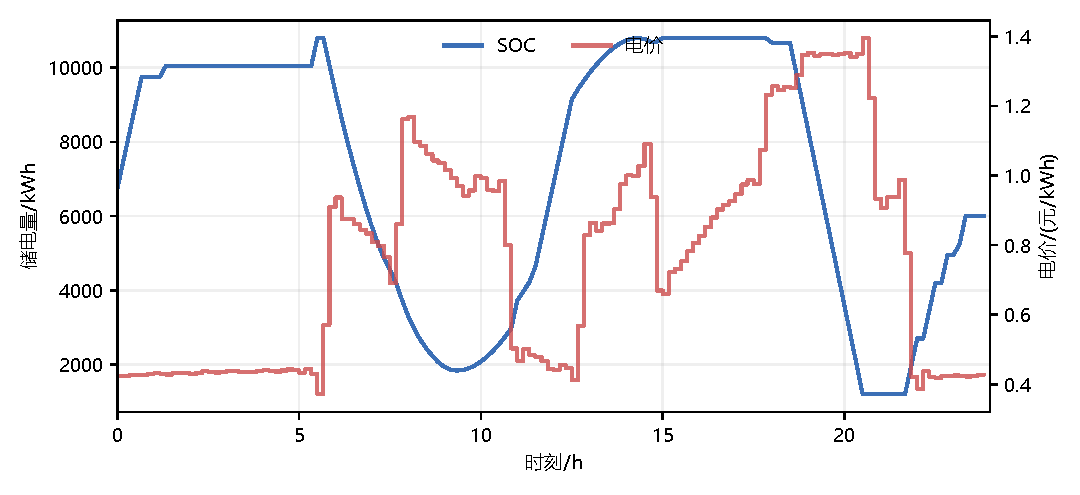
\includegraphics[width=0.88\textwidth]{../figures/p1_soc_price.pdf}
  \caption{问题一的储电量与分时电价}
  \label{fig:p1soc}
\end{figure}
